% Options for packages loaded elsewhere
% Options for packages loaded elsewhere
\PassOptionsToPackage{unicode}{hyperref}
\PassOptionsToPackage{hyphens}{url}
\PassOptionsToPackage{dvipsnames,svgnames,x11names}{xcolor}
%
\documentclass[
  letterpaper,
  DIV=11,
  numbers=noendperiod]{scrartcl}
\usepackage{xcolor}
\usepackage{amsmath,amssymb}
\setcounter{secnumdepth}{-\maxdimen} % remove section numbering
\usepackage{iftex}
\ifPDFTeX
  \usepackage[T1]{fontenc}
  \usepackage[utf8]{inputenc}
  \usepackage{textcomp} % provide euro and other symbols
\else % if luatex or xetex
  \usepackage{unicode-math} % this also loads fontspec
  \defaultfontfeatures{Scale=MatchLowercase}
  \defaultfontfeatures[\rmfamily]{Ligatures=TeX,Scale=1}
\fi
\usepackage{lmodern}
\ifPDFTeX\else
  % xetex/luatex font selection
\fi
% Use upquote if available, for straight quotes in verbatim environments
\IfFileExists{upquote.sty}{\usepackage{upquote}}{}
\IfFileExists{microtype.sty}{% use microtype if available
  \usepackage[]{microtype}
  \UseMicrotypeSet[protrusion]{basicmath} % disable protrusion for tt fonts
}{}
\makeatletter
\@ifundefined{KOMAClassName}{% if non-KOMA class
  \IfFileExists{parskip.sty}{%
    \usepackage{parskip}
  }{% else
    \setlength{\parindent}{0pt}
    \setlength{\parskip}{6pt plus 2pt minus 1pt}}
}{% if KOMA class
  \KOMAoptions{parskip=half}}
\makeatother
% Make \paragraph and \subparagraph free-standing
\makeatletter
\ifx\paragraph\undefined\else
  \let\oldparagraph\paragraph
  \renewcommand{\paragraph}{
    \@ifstar
      \xxxParagraphStar
      \xxxParagraphNoStar
  }
  \newcommand{\xxxParagraphStar}[1]{\oldparagraph*{#1}\mbox{}}
  \newcommand{\xxxParagraphNoStar}[1]{\oldparagraph{#1}\mbox{}}
\fi
\ifx\subparagraph\undefined\else
  \let\oldsubparagraph\subparagraph
  \renewcommand{\subparagraph}{
    \@ifstar
      \xxxSubParagraphStar
      \xxxSubParagraphNoStar
  }
  \newcommand{\xxxSubParagraphStar}[1]{\oldsubparagraph*{#1}\mbox{}}
  \newcommand{\xxxSubParagraphNoStar}[1]{\oldsubparagraph{#1}\mbox{}}
\fi
\makeatother


\usepackage{longtable,booktabs,array}
\usepackage{calc} % for calculating minipage widths
% Correct order of tables after \paragraph or \subparagraph
\usepackage{etoolbox}
\makeatletter
\patchcmd\longtable{\par}{\if@noskipsec\mbox{}\fi\par}{}{}
\makeatother
% Allow footnotes in longtable head/foot
\IfFileExists{footnotehyper.sty}{\usepackage{footnotehyper}}{\usepackage{footnote}}
\makesavenoteenv{longtable}
\usepackage{graphicx}
\makeatletter
\newsavebox\pandoc@box
\newcommand*\pandocbounded[1]{% scales image to fit in text height/width
  \sbox\pandoc@box{#1}%
  \Gscale@div\@tempa{\textheight}{\dimexpr\ht\pandoc@box+\dp\pandoc@box\relax}%
  \Gscale@div\@tempb{\linewidth}{\wd\pandoc@box}%
  \ifdim\@tempb\p@<\@tempa\p@\let\@tempa\@tempb\fi% select the smaller of both
  \ifdim\@tempa\p@<\p@\scalebox{\@tempa}{\usebox\pandoc@box}%
  \else\usebox{\pandoc@box}%
  \fi%
}
% Set default figure placement to htbp
\def\fps@figure{htbp}
\makeatother





\setlength{\emergencystretch}{3em} % prevent overfull lines

\providecommand{\tightlist}{%
  \setlength{\itemsep}{0pt}\setlength{\parskip}{0pt}}



 


\KOMAoption{captions}{tableheading}
\makeatletter
\@ifpackageloaded{caption}{}{\usepackage{caption}}
\AtBeginDocument{%
\ifdefined\contentsname
  \renewcommand*\contentsname{Table of contents}
\else
  \newcommand\contentsname{Table of contents}
\fi
\ifdefined\listfigurename
  \renewcommand*\listfigurename{List of Figures}
\else
  \newcommand\listfigurename{List of Figures}
\fi
\ifdefined\listtablename
  \renewcommand*\listtablename{List of Tables}
\else
  \newcommand\listtablename{List of Tables}
\fi
\ifdefined\figurename
  \renewcommand*\figurename{Figure}
\else
  \newcommand\figurename{Figure}
\fi
\ifdefined\tablename
  \renewcommand*\tablename{Table}
\else
  \newcommand\tablename{Table}
\fi
}
\@ifpackageloaded{float}{}{\usepackage{float}}
\floatstyle{ruled}
\@ifundefined{c@chapter}{\newfloat{codelisting}{h}{lop}}{\newfloat{codelisting}{h}{lop}[chapter]}
\floatname{codelisting}{Listing}
\newcommand*\listoflistings{\listof{codelisting}{List of Listings}}
\makeatother
\makeatletter
\makeatother
\makeatletter
\@ifpackageloaded{caption}{}{\usepackage{caption}}
\@ifpackageloaded{subcaption}{}{\usepackage{subcaption}}
\makeatother
\usepackage{bookmark}
\IfFileExists{xurl.sty}{\usepackage{xurl}}{} % add URL line breaks if available
\urlstyle{same}
\hypersetup{
  pdftitle={FIFA World Cup 2022 Scoring Efficiency Analysis - EDA},
  pdfauthor={Gaku Aihara and Jerry Xu},
  colorlinks=true,
  linkcolor={blue},
  filecolor={Maroon},
  citecolor={Blue},
  urlcolor={Blue},
  pdfcreator={LaTeX via pandoc}}


\title{FIFA World Cup 2022 Scoring Efficiency Analysis - EDA}
\author{Gaku Aihara and Jerry Xu}
\date{}
\begin{document}
\maketitle


\section{Exploratory Data Analysis}\label{exploratory-data-analysis}

\subsection{Introduction}\label{introduction}

This project studies scoring efficiency in the 2022 FIFA World Cup.
Specifically, we ask whether player-level statistics such as position,
age, playing time, shot volume, and shot quality can explain why some
players score more or fewer goals than expected. Our main outcome
variable is `xg\_diff`, defined as actual goals minus expected goals. A
positive value means a player overperformed their xG, while a negative
value means they underperformed.\\
\strut \\
This question is important because expected goals are widely used in
soccer analytics to evaluate player performance, but short tournaments
like the World Cup may contain a large amount of randomness. By
comparing exploratory visualizations with OLS, Ridge, and LASSO models,
we evaluate whether scoring efficiency can be explained by basic player
and shooting statistics.

\subsection{Data}\label{data}

Our primary dataset was gathered from Kaggle which originally gathered
data from FBRef, a widely used source for soccer statistics. We had
initially tried scraping from FBRef itself but the licensing would not
allow us to. The dataset contains 680 player-level observations from the
2022 FIFA World Cup, including key variables such as goals, expected
goals, age, position, team, and a variety of per-90 performance metrics.
We supplemented this with another Kaggle dataset that contained
shooting-specific information such as shot volume, shots on target,
average shot distance, and non-penalty xG per shot. These additional
variables allow us to better capture the quality and quantity of a
player's scoring opportunities, not just their outcomes.

\subsection{Exploring the Data}\label{exploring-the-data}

\textbf{What is your outcome variable(s)?}

Our outcome variable will be xg\_diff, the measurement of scoring
efficiency computed by taking the difference between Goals and xG.

\textbf{How well does it measure the outcome you are interested?}

This outcome variable measures how much a player converts relative to
the quality of their chances. We believe it is a reasonable proxy but
can be noisy with players who have low shot volume and xG models
themselves have errors.

\textbf{How does it relate to your expectations?}

We would expect forwards to show high variance while other positions to
cluster near zero. We would also expect younger, more creative players
to slightly overperform.

\textbf{What are your key explanatory variables?} - \emph{age\_years}:
player age - \emph{position}: player position (FW, MF, DF, GK) -
\emph{xG\_assist\_per90}: expected goals assisted per 90 minutes,
capturing a players playmaking contributions normalized for playing
time. - \emph{minutes\_90s}: measurement of the amount of playing time a
player gets relative to games - \emph{shots}: total number of shot
attempts a player has made throughout the tournament -
\emph{shots\_on\_target}: total number of shot attempts by a player that
was within the goal frame - \emph{goals\_per\_shot}: the ratio of goals
scored to total shots taken - \emph{average\_shot\_distance}: the
average shot distance of all the shots taken by a single player -
\emph{np\_xg\_per\_shot}: describes the quality of the shot by measuring
the non-penalty expected goal per shot

\subsection{Data Cleaning and
Transformation}\label{data-cleaning-and-transformation}

The raw dataset contained 680 player observations from the 2022 FIFA
World Cup.

\textbf{Filtering:} We removed players with fewer than 1 full 90-minute
equivalent play time and also dropped rows with missing values in xg,
goals, position, and age\_years. After doing this, we remained with 485
observations.

\textbf{New variables:} Our primary outcome variable, xg\_diff, was
created by subtracting a player's xG from their actual goals. A positive
value indicates overperformance while a negative value indicates
underperformance. Lastly, the is\_overperformer variable was created
taking value 1 if a player scored more than their xG and 0 otherwise.

\textbf{Age-parsing:} The age variable was stored as a character string
``years-days'' format so we extracted only the years as an integer.

\subsubsection{Figure 1}\label{figure-1}

\pandocbounded{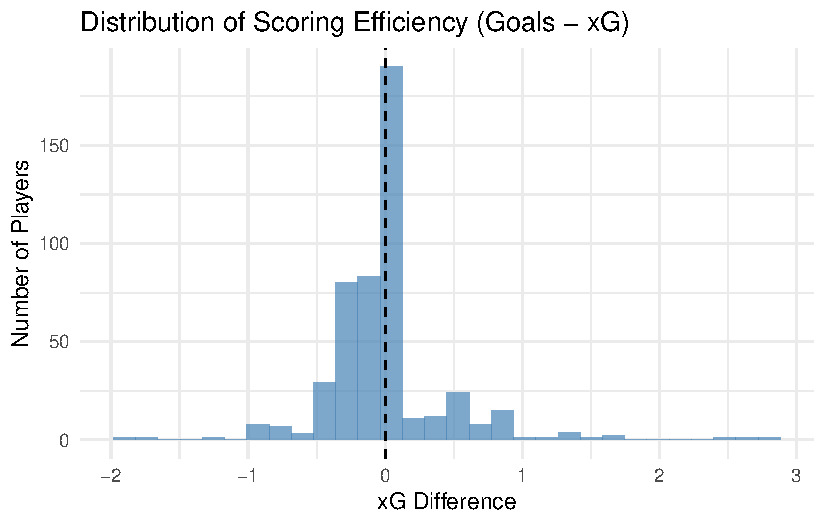
\includegraphics[keepaspectratio]{EDAupdate_files/figure-pdf/unnamed-chunk-4-1.pdf}}

The distribution shows that most players cluster around zero, indicating
that players generally perform close to their expected goals. There is a
slight right tail, indicating that a smaller number of players
significantly outperform their xG. Overall, extreme overperformers and
underperformers are relatively rare.

\subsubsection{Figure 2}\label{figure-2}

\pandocbounded{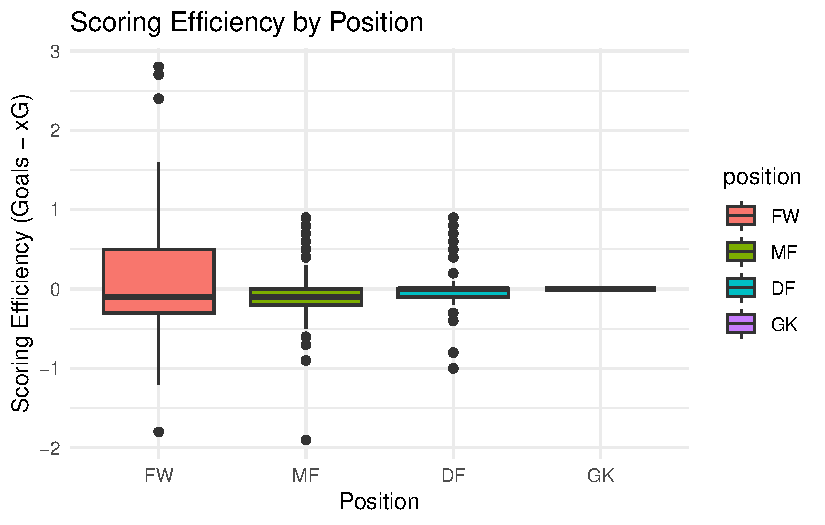
\includegraphics[keepaspectratio]{EDAupdate_files/figure-pdf/unnamed-chunk-5-1.pdf}}

This boxplot shows that forwards tend to have a wider spread and
slightly higher median efficiency compared to other positions. Defenders
and midfielders are generally centered around zero, suggesting they
perform closer to expectations. Goalkeepers show no variation since they
rarely score, so their efficiency remains near zero.

\subsubsection{Figure 3}\label{figure-3}

\pandocbounded{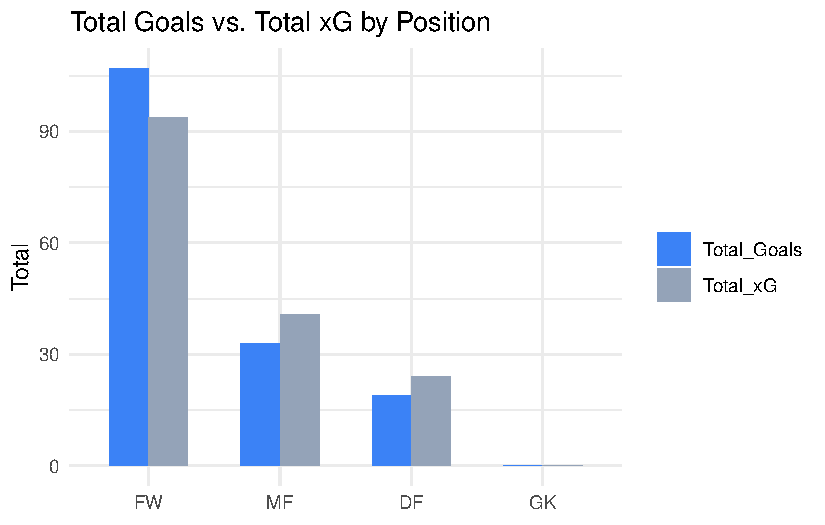
\includegraphics[keepaspectratio]{EDAupdate_files/figure-pdf/unnamed-chunk-6-1.pdf}}

This Bar Chart reveals that midfielders and defenders actually
underperform their xG while forwards overperform. We also notice that
both goals and xg is nonexistent for goalkeepers, indicating that the GK
position is irrelevant to our interest of study. These findings suggest
that position is a meaningful predictor of xg\_diff.

\subsubsection{Figure 4}\label{figure-4}

\pandocbounded{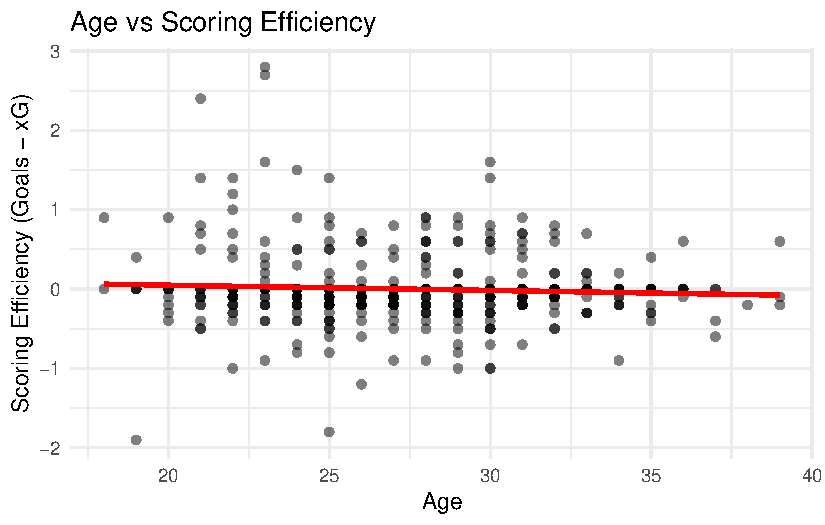
\includegraphics[keepaspectratio]{EDAupdate_files/figure-pdf/unnamed-chunk-7-1.pdf}}

This suggests that age is not a strong predictor of scoring efficiency
in this dataset, as points are widely scattered across all ages. Both
younger and older players can either overperform or underperform their
xG. This suggests that age is not a strong predictor of scoring
efficiency in this dataset.

\subsubsection{Figure 5}\label{figure-5}

\pandocbounded{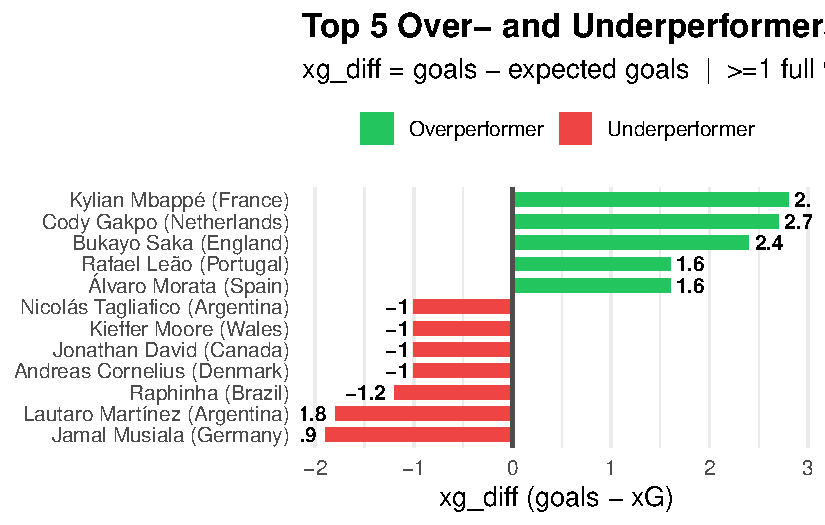
\includegraphics[keepaspectratio]{EDAupdate_files/figure-pdf/unnamed-chunk-8-1.pdf}}

This horizontal bar chart highlights the players who differentiated the
greatest from their statistical expectations. An observation is that all
overperformers were led by forwards including the top goal scorer of the
tournament Kylian Mbappe. This typically means these players have
exceptional finishing abilities scoring from difficult angles/distances.
The underscorers on the other hand are a mix of forwards, midfielders,
and even defenders. This indicates that players like Jamal Musiala and
Lautaro Martinez, who sit at the bottom, were frequently in good scoring
positions but struggled with their final touch or encountered
exceptional goalkeeping.

\subsubsection{Figure 6}\label{figure-6}

\pandocbounded{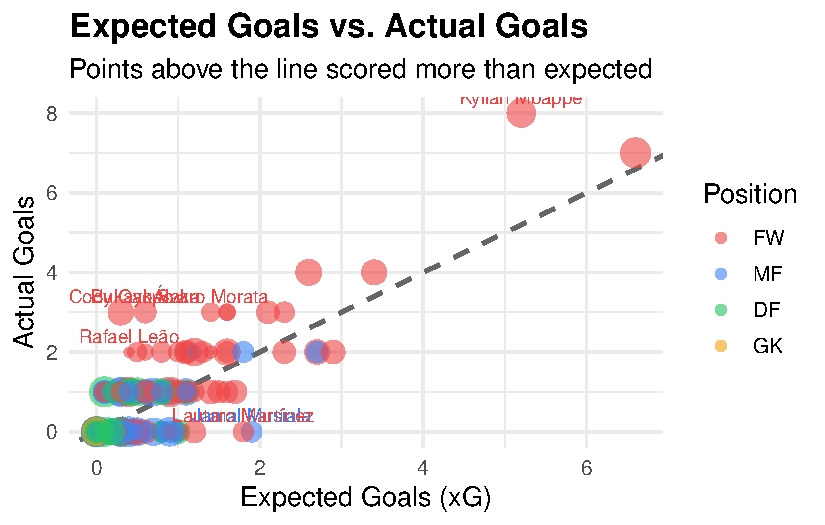
\includegraphics[keepaspectratio]{EDAupdate_files/figure-pdf/unnamed-chunk-9-1.pdf}}

This xG vs Actual goals scatter plot provides a broader view of player
efficiency across different positions (Fowards, Midfielders, Defenders,
Goalkeepers). The dashed line represents the break-even point where
players over the line overperformed and players under the line
underperformed. Again, a key outlier is Kylian Mbappe representing the
highest expected goal (roughly 5.2) and highest actual goal count (8).
There is a clear cluster of observations near the origin which
represents the limited scoring opportunities, primarily consisting of
defenders and midfielders. The overall trend seems to be that majority
of the high-volume scorers are forwards.

\subsubsection{Figure 7}\label{figure-7}

\pandocbounded{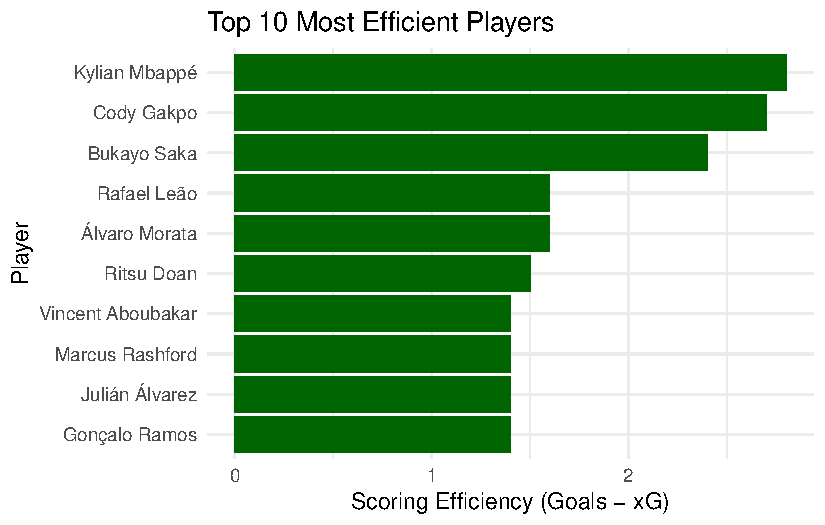
\includegraphics[keepaspectratio]{EDAupdate_files/figure-pdf/unnamed-chunk-10-1.pdf}}

This bar chart highlights the players who most exceeded their expected
goals during the tournament. Kylian Mbappé stands out as the most
efficient scorer, significantly outperforming his xG compared to others.
The remaining players also show strong positive efficiency, indicating
exceptional finishing performance.

\subsubsection{Figure 8}\label{figure-8}

\pandocbounded{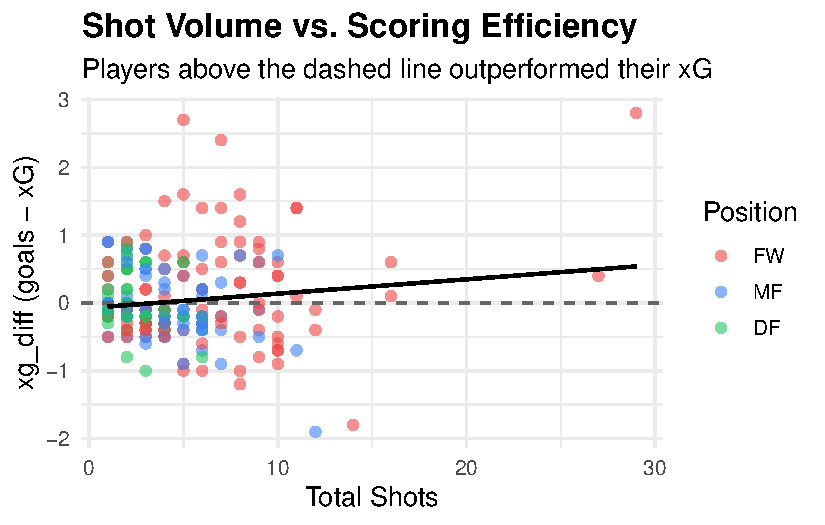
\includegraphics[keepaspectratio]{EDAupdate_files/figure-pdf/unnamed-chunk-11-1.pdf}}

This figure compares the total amount of shots of each player with
shooting efficiency. Each plot represents a single player and they are
color coded by positions. The dotted line at 0 defines the margin where
players above the line overperformed their expected goals and players
below the line underperformed. Looking at the plot, many of the extreme
overperformers cluster in the low to mid shot range (roughly 5-15),
meaning the biggest positive surprise came from players who didn't take
many shots. The players with the most shots consist entirely of
forwards, which are evenly spread above and below zero. This suggests
that high shot volume doesn't necessarily guarantee outperforming xG.
Lastly, midfielders and defenders cluster around 0 which is not
surprising because they rarely get as many opportunities as forwards to
attack the goal.

\subsubsection{Figure 9}\label{figure-9}

\pandocbounded{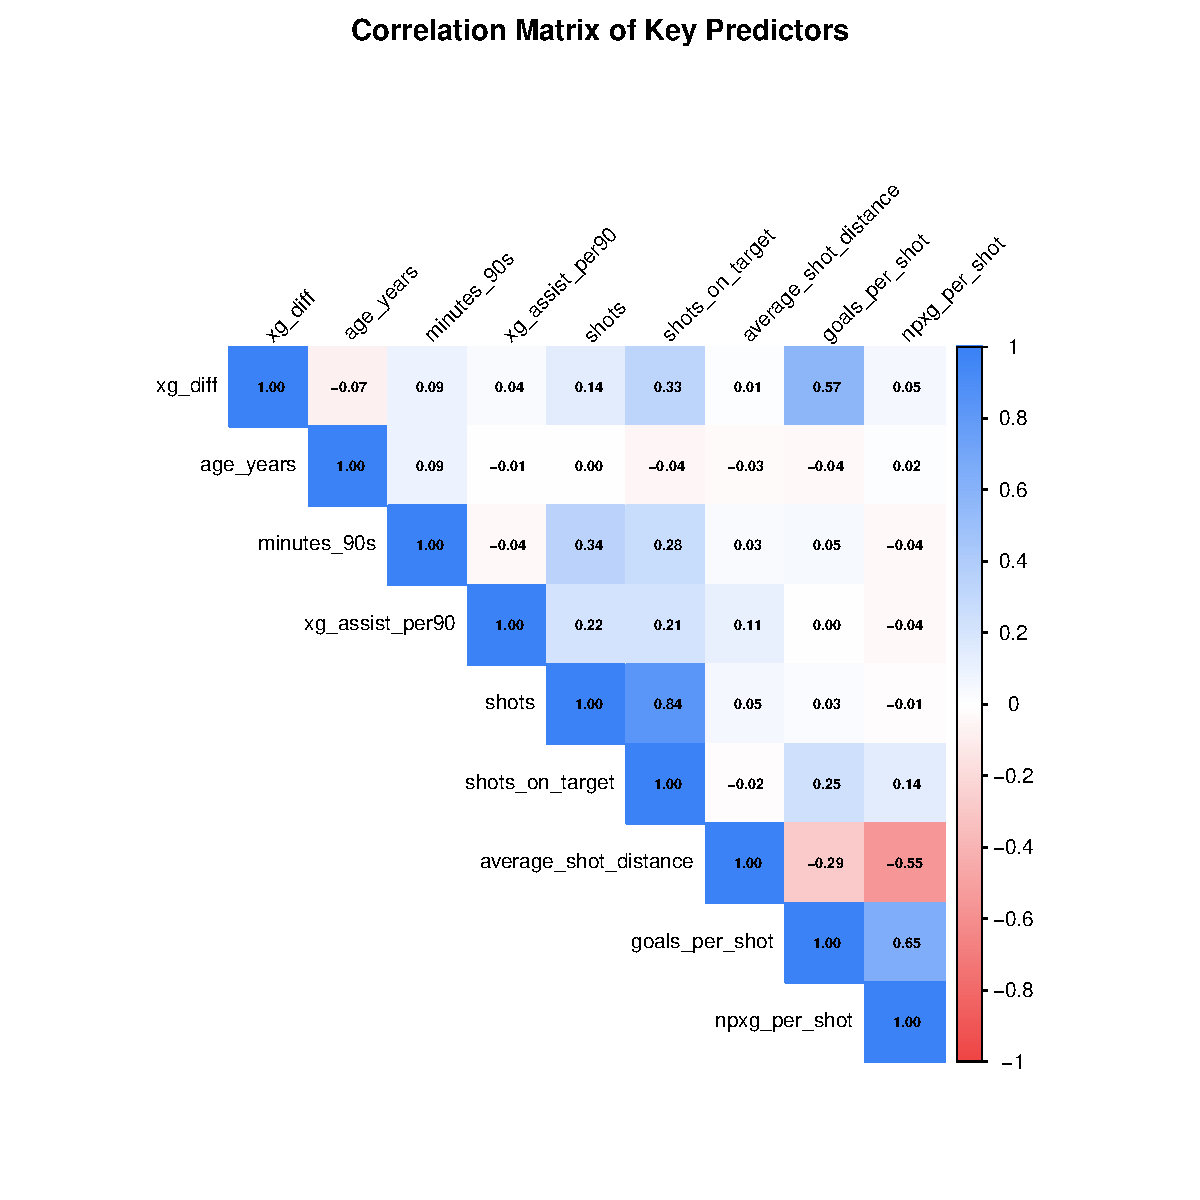
\includegraphics[keepaspectratio]{EDAupdate_files/figure-pdf/unnamed-chunk-12-1.pdf}}

This correlation plot visualizes the pairwise relationships between our
outcome variable and all predictor variables. The most notable finding
with respect to \emph{xg\_diff} is its strong positive correlation with
\emph{goals\_per\_shot} (\(0.57\)). This makes intuitive sense because
players who convert a higher fraction of their shots directly score more
goals relative to their xG. The second highest predictor is
\emph{shots\_on\_target} (\(0.33\)), suggesting that shot accuracy is
more predictive of outperforming xG than raw shot volume. Interestingly,
\emph{shots} itself only correlates at \(0.14\) with our outcome
variable, reinforcing that taking more shots does not guarantee
overperformance.Almost every other predictor variable is near zero
relative to our \emph{xg\_diff}. One notable relationship not involving
\emph{xg\_diff} is the strong positive correlation (\(0.84\)) between
\emph{shots} and \emph{shots\_on\_target}. This suggests
multicollinearity and including both variables in the model would not be
optimal. Similarly, \emph{goals\_per\_shot} and \emph{npxg\_per\_shot}
have a strong positive correlation of \(0.65\), and
\emph{average\_shot\_distance} negatively correlates with
\emph{npxg\_per\_shot} at \(-0.55\), confirming that shots taken from
farther away are of low quality.

\subsubsection{Data Summary}\label{data-summary}

\begin{verbatim}
     goals              xg           xg_diff             age_years    
 Min.   :0.0000   Min.   :0.000   Min.   :-1.9000000   Min.   :18.00  
 1st Qu.:0.0000   1st Qu.:0.000   1st Qu.:-0.2000000   1st Qu.:24.00  
 Median :0.0000   Median :0.100   Median : 0.0000000   Median :27.00  
 Mean   :0.3278   Mean   :0.327   Mean   : 0.0008247   Mean   :27.34  
 3rd Qu.:0.0000   3rd Qu.:0.400   3rd Qu.: 0.0000000   3rd Qu.:30.00  
 Max.   :8.0000   Max.   :6.600   Max.   : 2.8000000   Max.   :39.00  
                                                                      
     shots         minutes_90s    xg_assist_per90   average_shot_distance
 Min.   : 0.000   Min.   :1.000   Min.   :0.00000   Min.   : 0.90        
 1st Qu.: 0.000   1st Qu.:1.700   1st Qu.:0.00000   1st Qu.:11.50        
 Median : 2.000   Median :2.800   Median :0.03000   Median :16.50        
 Mean   : 2.691   Mean   :2.803   Mean   :0.08371   Mean   :17.44        
 3rd Qu.: 4.000   3rd Qu.:3.400   3rd Qu.:0.11000   3rd Qu.:22.40        
 Max.   :29.000   Max.   :7.700   Max.   :1.44000   Max.   :46.60        
                                                    NA's   :124          
 npxg_per_shot   
 Min.   :0.0100  
 1st Qu.:0.0400  
 Median :0.0800  
 Mean   :0.1094  
 3rd Qu.:0.1300  
 Max.   :0.9600  
 NA's   :124     
\end{verbatim}

\begin{longtable}[]{@{}ll@{}}
\caption{Data summary}\tabularnewline
\toprule\noalign{}
\endfirsthead
\endhead
\bottomrule\noalign{}
\endlastfoot
Name & df \\
Number of rows & 485 \\
Number of columns & 40 \\
\_\_\_\_\_\_\_\_\_\_\_\_\_\_\_\_\_\_\_\_\_\_\_ & \\
Column type frequency: & \\
character & 4 \\
factor & 1 \\
numeric & 35 \\
\_\_\_\_\_\_\_\_\_\_\_\_\_\_\_\_\_\_\_\_\_\_\_\_ & \\
Group variables & None \\
\end{longtable}

\textbf{Variable type: character}

\begin{longtable}[]{@{}
  >{\raggedright\arraybackslash}p{(\linewidth - 14\tabcolsep) * \real{0.1944}}
  >{\raggedleft\arraybackslash}p{(\linewidth - 14\tabcolsep) * \real{0.1389}}
  >{\raggedleft\arraybackslash}p{(\linewidth - 14\tabcolsep) * \real{0.1944}}
  >{\raggedleft\arraybackslash}p{(\linewidth - 14\tabcolsep) * \real{0.0556}}
  >{\raggedleft\arraybackslash}p{(\linewidth - 14\tabcolsep) * \real{0.0556}}
  >{\raggedleft\arraybackslash}p{(\linewidth - 14\tabcolsep) * \real{0.0833}}
  >{\raggedleft\arraybackslash}p{(\linewidth - 14\tabcolsep) * \real{0.1250}}
  >{\raggedleft\arraybackslash}p{(\linewidth - 14\tabcolsep) * \real{0.1528}}@{}}
\toprule\noalign{}
\begin{minipage}[b]{\linewidth}\raggedright
skim\_variable
\end{minipage} & \begin{minipage}[b]{\linewidth}\raggedleft
n\_missing
\end{minipage} & \begin{minipage}[b]{\linewidth}\raggedleft
complete\_rate
\end{minipage} & \begin{minipage}[b]{\linewidth}\raggedleft
min
\end{minipage} & \begin{minipage}[b]{\linewidth}\raggedleft
max
\end{minipage} & \begin{minipage}[b]{\linewidth}\raggedleft
empty
\end{minipage} & \begin{minipage}[b]{\linewidth}\raggedleft
n\_unique
\end{minipage} & \begin{minipage}[b]{\linewidth}\raggedleft
whitespace
\end{minipage} \\
\midrule\noalign{}
\endhead
\bottomrule\noalign{}
\endlastfoot
player & 0 & 1 & 4 & 26 & 0 & 485 & 0 \\
team & 0 & 1 & 5 & 14 & 0 & 32 & 0 \\
age & 0 & 1 & 6 & 6 & 0 & 459 & 0 \\
club & 0 & 1 & 4 & 33 & 0 & 203 & 0 \\
\end{longtable}

\textbf{Variable type: factor}

\begin{longtable}[]{@{}
  >{\raggedright\arraybackslash}p{(\linewidth - 10\tabcolsep) * \real{0.1573}}
  >{\raggedleft\arraybackslash}p{(\linewidth - 10\tabcolsep) * \real{0.1124}}
  >{\raggedleft\arraybackslash}p{(\linewidth - 10\tabcolsep) * \real{0.1573}}
  >{\raggedright\arraybackslash}p{(\linewidth - 10\tabcolsep) * \real{0.0899}}
  >{\raggedleft\arraybackslash}p{(\linewidth - 10\tabcolsep) * \real{0.1011}}
  >{\raggedright\arraybackslash}p{(\linewidth - 10\tabcolsep) * \real{0.3820}}@{}}
\toprule\noalign{}
\begin{minipage}[b]{\linewidth}\raggedright
skim\_variable
\end{minipage} & \begin{minipage}[b]{\linewidth}\raggedleft
n\_missing
\end{minipage} & \begin{minipage}[b]{\linewidth}\raggedleft
complete\_rate
\end{minipage} & \begin{minipage}[b]{\linewidth}\raggedright
ordered
\end{minipage} & \begin{minipage}[b]{\linewidth}\raggedleft
n\_unique
\end{minipage} & \begin{minipage}[b]{\linewidth}\raggedright
top\_counts
\end{minipage} \\
\midrule\noalign{}
\endhead
\bottomrule\noalign{}
\endlastfoot
position & 0 & 1 & FALSE & 4 & DF: 183, MF: 144, FW: 119, GK: 39 \\
\end{longtable}

\textbf{Variable type: numeric}

\begin{longtable}[]{@{}
  >{\raggedright\arraybackslash}p{(\linewidth - 20\tabcolsep) * \real{0.2273}}
  >{\raggedleft\arraybackslash}p{(\linewidth - 20\tabcolsep) * \real{0.0909}}
  >{\raggedleft\arraybackslash}p{(\linewidth - 20\tabcolsep) * \real{0.1273}}
  >{\raggedleft\arraybackslash}p{(\linewidth - 20\tabcolsep) * \real{0.0727}}
  >{\raggedleft\arraybackslash}p{(\linewidth - 20\tabcolsep) * \real{0.0636}}
  >{\raggedleft\arraybackslash}p{(\linewidth - 20\tabcolsep) * \real{0.0727}}
  >{\raggedleft\arraybackslash}p{(\linewidth - 20\tabcolsep) * \real{0.0727}}
  >{\raggedleft\arraybackslash}p{(\linewidth - 20\tabcolsep) * \real{0.0727}}
  >{\raggedleft\arraybackslash}p{(\linewidth - 20\tabcolsep) * \real{0.0727}}
  >{\raggedleft\arraybackslash}p{(\linewidth - 20\tabcolsep) * \real{0.0727}}
  >{\raggedright\arraybackslash}p{(\linewidth - 20\tabcolsep) * \real{0.0545}}@{}}
\toprule\noalign{}
\begin{minipage}[b]{\linewidth}\raggedright
skim\_variable
\end{minipage} & \begin{minipage}[b]{\linewidth}\raggedleft
n\_missing
\end{minipage} & \begin{minipage}[b]{\linewidth}\raggedleft
complete\_rate
\end{minipage} & \begin{minipage}[b]{\linewidth}\raggedleft
mean
\end{minipage} & \begin{minipage}[b]{\linewidth}\raggedleft
sd
\end{minipage} & \begin{minipage}[b]{\linewidth}\raggedleft
p0
\end{minipage} & \begin{minipage}[b]{\linewidth}\raggedleft
p25
\end{minipage} & \begin{minipage}[b]{\linewidth}\raggedleft
p50
\end{minipage} & \begin{minipage}[b]{\linewidth}\raggedleft
p75
\end{minipage} & \begin{minipage}[b]{\linewidth}\raggedleft
p100
\end{minipage} & \begin{minipage}[b]{\linewidth}\raggedright
hist
\end{minipage} \\
\midrule\noalign{}
\endhead
\bottomrule\noalign{}
\endlastfoot
birth\_year & 0 & 1.00 & 1994.63 & 4.15 & 1983.00 & 1992.00 & 1995.00 &
1998.00 & 2004.00 & ▁▅▇▇▃ \\
games & 0 & 1.00 & 3.48 & 1.40 & 1.00 & 3.00 & 3.00 & 4.00 & 7.00 &
▃▇▅▂▂ \\
games\_starts & 0 & 1.00 & 2.80 & 1.53 & 0.00 & 2.00 & 3.00 & 4.00 &
7.00 & ▃▃▇▁▁ \\
minutes & 0 & 1.00 & 252.37 & 131.50 & 86.00 & 151.00 & 249.00 & 310.00
& 690.00 & ▇▇▃▁▁ \\
minutes\_90s & 0 & 1.00 & 2.80 & 1.46 & 1.00 & 1.70 & 2.80 & 3.40 & 7.70
& ▇▇▃▁▁ \\
goals & 0 & 1.00 & 0.33 & 0.80 & 0.00 & 0.00 & 0.00 & 0.00 & 8.00 &
▇▁▁▁▁ \\
assists & 0 & 1.00 & 0.24 & 0.56 & 0.00 & 0.00 & 0.00 & 0.00 & 3.00 &
▇▂▁▁▁ \\
goals\_pens & 0 & 1.00 & 0.29 & 0.68 & 0.00 & 0.00 & 0.00 & 0.00 & 6.00
& ▇▁▁▁▁ \\
pens\_made & 0 & 1.00 & 0.04 & 0.25 & 0.00 & 0.00 & 0.00 & 0.00 & 4.00 &
▇▁▁▁▁ \\
pens\_att & 0 & 1.00 & 0.05 & 0.31 & 0.00 & 0.00 & 0.00 & 0.00 & 5.00 &
▇▁▁▁▁ \\
cards\_yellow & 0 & 1.00 & 0.41 & 0.61 & 0.00 & 0.00 & 0.00 & 1.00 &
3.00 & ▇▃▁▁▁ \\
cards\_red & 0 & 1.00 & 0.01 & 0.08 & 0.00 & 0.00 & 0.00 & 0.00 & 1.00 &
▇▁▁▁▁ \\
goals\_per90 & 0 & 1.00 & 0.12 & 0.29 & 0.00 & 0.00 & 0.00 & 0.00 & 2.05
& ▇▁▁▁▁ \\
assists\_per90 & 0 & 1.00 & 0.08 & 0.19 & 0.00 & 0.00 & 0.00 & 0.00 &
1.19 & ▇▁▁▁▁ \\
goals\_assists\_per90 & 0 & 1.00 & 0.20 & 0.37 & 0.00 & 0.00 & 0.00 &
0.33 & 2.37 & ▇▁▁▁▁ \\
goals\_pens\_per90 & 0 & 1.00 & 0.11 & 0.28 & 0.00 & 0.00 & 0.00 & 0.00
& 2.05 & ▇▁▁▁▁ \\
goals\_assists\_pens\_per90 & 0 & 1.00 & 0.19 & 0.36 & 0.00 & 0.00 &
0.00 & 0.33 & 2.37 & ▇▁▁▁▁ \\
xg & 0 & 1.00 & 0.33 & 0.60 & 0.00 & 0.00 & 0.10 & 0.40 & 6.60 &
▇▁▁▁▁ \\
npxg & 0 & 1.00 & 0.29 & 0.46 & 0.00 & 0.00 & 0.10 & 0.40 & 3.60 &
▇▁▁▁▁ \\
xg\_assist & 0 & 1.00 & 0.22 & 0.36 & 0.00 & 0.00 & 0.10 & 0.30 & 3.10 &
▇▁▁▁▁ \\
npxg\_xg\_assist & 0 & 1.00 & 0.51 & 0.67 & 0.00 & 0.10 & 0.30 & 0.70 &
5.10 & ▇▁▁▁▁ \\
xg\_per90 & 0 & 1.00 & 0.13 & 0.20 & 0.00 & 0.00 & 0.05 & 0.14 & 1.19 &
▇▁▁▁▁ \\
xg\_assist\_per90 & 0 & 1.00 & 0.08 & 0.14 & 0.00 & 0.00 & 0.03 & 0.11 &
1.44 & ▇▁▁▁▁ \\
xg\_xg\_assist\_per90 & 0 & 1.00 & 0.21 & 0.26 & 0.00 & 0.03 & 0.12 &
0.28 & 1.54 & ▇▂▁▁▁ \\
npxg\_per90 & 0 & 1.00 & 0.12 & 0.18 & 0.00 & 0.00 & 0.05 & 0.13 & 1.19
& ▇▁▁▁▁ \\
npxg\_xg\_assist\_per90 & 0 & 1.00 & 0.20 & 0.25 & 0.00 & 0.03 & 0.12 &
0.27 & 1.54 & ▇▂▁▁▁ \\
xg\_diff & 0 & 1.00 & 0.00 & 0.44 & -1.90 & -0.20 & 0.00 & 0.00 & 2.80 &
▁▆▇▁▁ \\
efficiency\_per90 & 0 & 1.00 & -0.01 & 0.20 & -1.00 & -0.06 & -0.01 &
0.00 & 1.63 & ▁▇▂▁▁ \\
age\_years & 0 & 1.00 & 27.34 & 4.15 & 18.00 & 24.00 & 27.00 & 30.00 &
39.00 & ▃▇▇▅▁ \\
is\_overperformer & 0 & 1.00 & 0.18 & 0.39 & 0.00 & 0.00 & 0.00 & 0.00 &
1.00 & ▇▁▁▁▂ \\
shots & 0 & 1.00 & 2.69 & 3.34 & 0.00 & 0.00 & 2.00 & 4.00 & 29.00 &
▇▂▁▁▁ \\
shots\_on\_target & 0 & 1.00 & 0.89 & 1.50 & 0.00 & 0.00 & 0.00 & 1.00 &
13.00 & ▇▁▁▁▁ \\
average\_shot\_distance & 124 & 0.74 & 17.44 & 7.24 & 0.90 & 11.50 &
16.50 & 22.40 & 46.60 & ▂▇▅▂▁ \\
goals\_per\_shot & 124 & 0.74 & 0.10 & 0.21 & 0.00 & 0.00 & 0.00 & 0.11
& 1.00 & ▇▁▁▁▁ \\
npxg\_per\_shot & 124 & 0.74 & 0.11 & 0.12 & 0.01 & 0.04 & 0.08 & 0.13 &
0.96 & ▇▁▁▁▁ \\
\end{longtable}

\subsection{Modeling(Methodology)}\label{modelingmethodology}

We model \emph{xg\_diff} (scoring efficiency computed as goals -
expected goals) as a function of player age, position, playing time,
playmaking context, shot volume, shot distance, and shot quality. We
excluded goalkeepers from all models as they are not meaningful for
scoring analysis. We also exclude \emph{goals\_per\_shot} and
\emph{shots\_on\_target} from predictors due to the high correlation we
found from the correlation matrix. All three models (OLS, Ridge, LASSO)
are evaluated using 10-fold cross-validation with both RMSE and MAE as
performance metrics.

Our model is specified as:

\[xg\_diff = \beta_0 + \beta_1(age\_years) + \beta_2(position) + \beta_3(minutes\_90s) + \\\beta_4(xg\_assist\_per90) + \beta_5(shots) + \beta_6(average\_shot\_distance) + \\\beta_7(npxg\_per\_shot) + \varepsilon\]

\subsubsection{OLS}\label{ols}

\begin{longtable}[]{@{}lrrrr@{}}
\caption{OLS Coefficients (R² = 0.048)}\tabularnewline
\toprule\noalign{}
term & estimate & std.error & statistic & p.value \\
\midrule\noalign{}
\endfirsthead
\toprule\noalign{}
term & estimate & std.error & statistic & p.value \\
\midrule\noalign{}
\endhead
\bottomrule\noalign{}
\endlastfoot
(Intercept) & 0.1178 & 0.2134 & 0.5521 & 0.5812 \\
age\_years & -0.0096 & 0.0066 & -1.4522 & 0.1473 \\
positionMF & -0.1752 & 0.0738 & -2.3732 & 0.0182 \\
positionDF & -0.1346 & 0.0804 & -1.6746 & 0.0949 \\
minutes\_90s & 0.0351 & 0.0213 & 1.6489 & 0.1001 \\
xg\_assist\_per90 & 0.0082 & 0.1984 & 0.0413 & 0.9671 \\
shots & 0.0070 & 0.0101 & 0.6965 & 0.4866 \\
average\_shot\_distance & 0.0048 & 0.0046 & 1.0504 & 0.2943 \\
npxg\_per\_shot & 0.3476 & 0.2736 & 1.2704 & 0.2048 \\
\end{longtable}

The OLS model returns an \(R^2\) of \(0.048\), meaning our predictors
explain about \(4.8%
\) of the variance in \emph{xg\_diff}. This is extremely low but not too
surprising as it shows scoring efficiency is very noisy and difficult to
predict from player-level statistics alone. \emph{positionMF} was our
only statistically significant coefficient indicating that midfielders
on average score approximately 0.17 goals less than their xG relative to
forwards with all other variables held constant. \emph{positionDF} is
also marginally significant.

\subsubsection{Ridge}\label{ridge}

Ridge regression applies L2 regularization which penalizes the sum of
squares coefficients to shrink all predictors towards zero without
eliminating any. The optimal lambda selected by cross-validation is
0.3588 indicating moderate regularization strength.

\subsubsection{LASSO}\label{lasso}

LASSO regression applies L1 regularization which performs automatic
variable selection by shrinking selected coefficients to zero.

\begin{longtable}[]{@{}lrl@{}}
\caption{LASSO Coefficients (lambda = 0.004)}\tabularnewline
\toprule\noalign{}
Variable & Coefficient & Status \\
\midrule\noalign{}
\endfirsthead
\toprule\noalign{}
Variable & Coefficient & Status \\
\midrule\noalign{}
\endhead
\bottomrule\noalign{}
\endlastfoot
npxg\_per\_shot & 0.2735 & Retained \\
positionMF & -0.1514 & Retained \\
positionDF & -0.1139 & Retained \\
minutes\_90s & 0.0304 & Retained \\
age\_years & -0.0086 & Retained \\
shots & 0.0080 & Retained \\
average\_shot\_distance & 0.0034 & Retained \\
positionGK & 0.0000 & Zeroed Out \\
xg\_assist\_per90 & 0.0000 & Zeroed Out \\
\end{longtable}

With an optimal lamdba of \(0.004\), LASSO zeroed out \emph{positionGK}
and \emph{xg\_assist\_per90}. The first variable makes sense as
goalkeepers do not contribute to scoring goals but the creativity metric
being zeroed out is a surprise. \emph{np\_xg\_per\_shot} is retained
with the largest magnitude coefficient (\(0.2735\)). The two position
dummies (\emph{positionMF}, \emph{positionDF}) are retained and have
negative coefficients, reinforcing that non-forward positions tend to
underperform their xG. The remaining retained variables
(\emph{minutes\_90s}, \emph{age\_years}, \emph{shots},
\emph{average\_shot\_distance}) all have very small coefficients,
suggesting their contribution is minimal but non-negligible after
regularization.

\begin{longtable}[]{@{}lrrr@{}}
\caption{10-Fold CV Performance Across Models}\tabularnewline
\toprule\noalign{}
Model & CV RMSE & CV MAE & Optimal Lambda \\
\midrule\noalign{}
\endfirsthead
\toprule\noalign{}
Model & CV RMSE & CV MAE & Optimal Lambda \\
\midrule\noalign{}
\endhead
\bottomrule\noalign{}
\endlastfoot
OLS & 0.5122 & 0.3297 & NA \\
Ridge & 0.5093 & 0.3262 & 0.3588 \\
LASSO & 0.5110 & 0.3287 & 0.0040 \\
\end{longtable}

Ridge regression receives the lowest CV RMSE and CV MAE, making it the
best performing model on both metrics. However, the difference across
all three models are very small indicating that regularization provides
little benefit over the standard OLS. This likely reflects the fact that
our predictors are already weakly correlated with \emph{xg\_diff} so
there is little to gain from shrinkage. Overall, while Ridge edges out
the other methods, all three models suggest that the selected predictors
have limited power in explaining scoring efficiency, and future modeling
could benefit from additional data sources.

\subsection{Results}\label{results}

The exploratory analysis shows that most players had an `xg\_diff` close
to zero, meaning most players scored near their expected goals. However,
a small number of players strongly overperformed or underperformed.
Position appeared to matter more than age or raw shot volume. Forwards
had the widest spread in scoring efficiency and included most of the top
overperformers, while midfielders and defenders tended to cluster closer
to zero or slightly below zero.\\
\strut \\
The correlation matrix showed that `goals\_per\_shot` had the strongest
correlation with `xg\_diff`, followed by `shots\_on\_target`. However,
these variables were excluded from the final models because they are
closely related to the outcome or highly correlated with other shooting
variables. Other predictors, including age, minutes, shots, and average
shot distance, had weak relationships with scoring efficiency.\\
\strut \\
The OLS model had an \textbackslash(R\^{}2\textbackslash) of 0.048,
meaning the model explained only about 4.8\% of the variation in scoring
efficiency. This suggests that the selected player-level variables have
limited explanatory power. Ridge regression had the best cross-validated
RMSE and MAE, but the difference between OLS, Ridge, and LASSO was very
small. Overall, the modeling results suggest that scoring efficiency in
a short tournament is difficult to predict using only basic player and
shooting statistics.

\subsection{Discussion}\label{discussion}

Our analysis suggests that scoring efficiency in the 2022 FIFA World Cup
is difficult to predict using basic player-level and shooting statistics
alone. Although some variables are related to overperformance, most
predictors have weak relationships with `xg\_diff`, which supports the
idea that finishing above or below expected goals is highly noisy in a
short tournament setting. The distribution of `xg\_diff` shows that most
players finished close to their expected goals, while only a small
number of players strongly overperformed or underperformed.\\
\strut \\
Position appears to be one of the most meaningful factors in our
analysis. Forwards had the widest spread in scoring efficiency and were
more likely to appear among the strongest overperformers. This makes
sense because forwards take more shots and are usually the primary
goal-scoring players on their teams. Midfielders and defenders tended to
cluster closer to zero or slightly below zero, suggesting that they
generally scored closer to or below expectation. Goalkeepers were not
meaningful for this research question because they rarely produce
scoring opportunities, so excluding them from the modeling stage was
appropriate.\\
\strut \\
The relationship between age and scoring efficiency was weak. Players of
different ages appeared on both sides of the overperformance line, which
suggests that age alone is not a strong predictor of whether a player
will score more than expected. Similarly, total shot volume was not
strongly associated with overperforming xG. Some players with many shots
still underperformed, while some of the largest overperformers came from
low or medium shot volume. This suggests that simply taking more shots
does not guarantee better finishing efficiency.\\
\strut \\
The correlation matrix gave more useful insight into which variables
were most connected to scoring efficiency. `goals\_per\_shot` had the
strongest positive correlation with `xg\_diff`, which is intuitive
because players who score on a higher percentage of their shots are more
likely to outperform their xG. `shots\_on\_target` was also positively
related to `xg\_diff`, suggesting that shot accuracy matters more than
raw shot quantity. However, we excluded `goals\_per\_shot` and
`shots\_on\_target` from the final models because they are highly
related to the outcome or strongly correlated with other shooting
variables, which could create multicollinearity or make the model less
interpretable.\\
\strut \\
The modeling results reinforce the main finding from the EDA: scoring
efficiency is difficult to explain with the variables available in this
dataset. The OLS model had an \textbackslash(R\^{}2\textbackslash) of
only 0.048, meaning the predictors explained about 4.8\% of the
variation in `xg\_diff`. Ridge regression performed slightly better than
OLS and LASSO based on cross-validated RMSE and MAE, but the differences
between the three models were very small. This indicates that
regularization did not substantially improve predictive performance.
LASSO retained variables such as `npxg\_per\_shot`, position, minutes,
age, shots, and average shot distance, but most coefficients were small,
again suggesting limited explanatory power.\\
\strut \\
One important limitation of this project is that the World Cup is a
small and short tournament. Many players have limited minutes and few
shots, so one goal or one missed chance can greatly change a player's
`xg\_diff`. This makes scoring efficiency much more unstable than it
would be across a full club season. Another limitation is that xG models
are not perfect. They estimate chance quality based on available
information, but they may not fully capture defensive pressure,
goalkeeper positioning, shot technique, tactical context, or game state.
Also, our dataset is player-level rather than shot-level, so we lose
detailed information about each individual chance.\\
\strut \\
Future work could improve this analysis by using shot-level data instead
of aggregated player-level statistics. Shot-level data would allow us to
include variables such as shot angle, body part used, defensive
pressure, pass type, match situation, and goalkeeper position. It would
also be useful to compare World Cup performance with players' club
performance across a full season to see whether overperformance in the
tournament reflects true finishing skill or short-term randomness.
Finally, adding team-level variables such as possession, attacking
style, and strength of opponents could help explain why some players
receive higher-quality chances than others.\\
\strut \\
Overall, our results suggest that scoring efficiency is not easily
predicted from simple player statistics. Position and shooting quality
provide some insight, but most of the variation in `xg\_diff` appears to
come from randomness, small sample size, and contextual factors not
captured in the dataset. This supports the idea that xG overperformance
in a short tournament should be interpreted carefully rather than
treated as a stable measure of finishing ability.

\subsection{Codebook}\label{codebook}

The codebook can be found in our GitHub in our data/ folder:
\url{https://github.com/zibojerryxu/Math-244-final-project-Team-GG/blob/main/data/dataset_readme.md}




\end{document}
